\section{Критическое поведение модели IsingISAW на треугольной решётке}

В данном разделе проводится исследование критической области модели Изинга на случайном блуждания без самопересечений на треугольной решётке (далее, TrIsingISAW).
В отличие от классической модели на квадратной решётке, узлы треугольной решётки имеют две дополнительные связи по одной из диагоналей (см. рисунок \ref{fig:lattices}), 
вследствие чего координационное число данной модификации (кол-во возможных связей у одного узла) увеличено по сравнению с квадратной с 4 до 6.

\subsection{Поиск точки фазового перехода}

\begin{equation}
\label{eq:IsISAW_H}
 H_{N,u,\{\sigma\}} = -\sum_{i,j} J\sigma_i \sigma_j, i,j \in u, |u| = N
\end{equation}

\begin{equation}
\label{eq:TrIsISAW_E}
\la \epsilon \ra = \la H \ra / N
\end{equation}

Были проведены симуляции Монте-Карло при нулевом внешнем поле и $J \in [0,0.9]$. 
Итоговое количество шагов симуляций от $10^10$ до $10^11$, симулированные блуждания имеют длину $N$ от 100 до 7200.
Были собраны данные для удельной энергии системы на спин $\la \epsilon \ra$ \eqref{eq:TrIsISAW_E} и средняя 2-я и 4-я степени намагниченности на спин $\la m^2 \ra$, $\la m^4 \ra$.
Так же собрана статистика среднего расстояния между концами блуждания $R^2_N$.

\begin{equation}
\label{eq:IsISAW_m2}
	m^{k} = (\sum_{i \in u} \sigma_i / N)^k
\end{equation}

\begin{figure}[h]
\begin{subfigure}{0.49\textwidth}
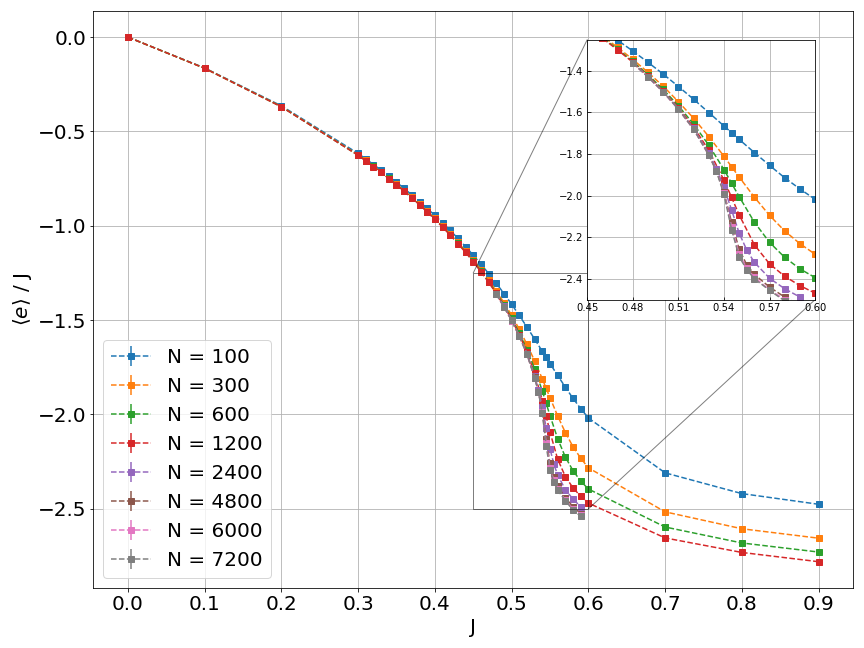
\includegraphics[width=\textwidth]{TrIsISAW_E.png}
\caption{}
\label{fig:TrIsISAW_E}
\end{subfigure}
\hfill
\begin{subfigure}{0.49\textwidth}
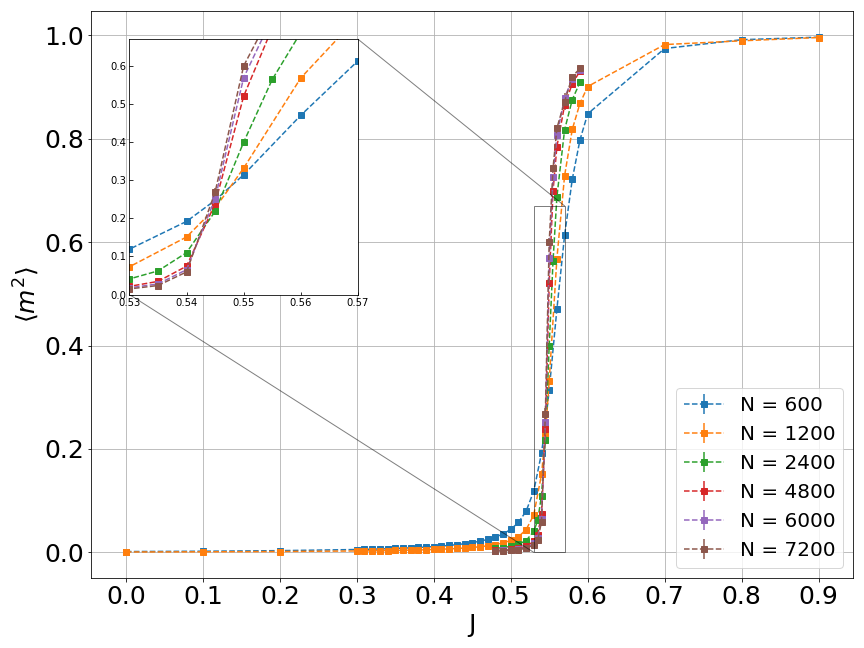
\includegraphics[width=\textwidth]{TrIsISAW_m2.png}
\caption{}
\label{fig:TrIsISAW_m2}
\end{subfigure}
\caption{Слева: удельная энергия узла \eqref{eq:TrIsISAW_E} модели TrIsingISAW (без учёта константы $J$).
Справа: средняя вторая степень намагниченности \eqref{eq:IsISAW_m2} узла модели TrIsingISAW. 
Длины конформаций в обоих графиках от 100 до 7200 (длины отмечены разными цветами)}

\end{figure}

На графике \ref{fig:TrIsISAW_E} показана зависимость удельной энергии \eqref{eq:TrIsISAW_E} узла модели TrIsingISAW.
График показывает что удельная энергия системы стремится к -3J в пределе бесконечной длины конформации, 
что логично, поскольку с ростом $J$ узлы приобретают наиболее возможное число связей (то есть, 6), но так как св
язи существуют между парами узлов,
необходимо поделить число связей на 2.
При малых $J$ энергия почти не зависит от длины цепочки $N$, но начиная с $J > 0.53$, расхождение графиков становится наиболее четким.

На графике \ref{fig:TrIsISAW_m2} изображен момент намагниченности второго порядка \eqref{eq:IsISAW_m2} в зависимости от $J$.
Графики величины для конформаций разных длин имеют четкое пересечение в $J \approx 0.545$.

\begin{equation}
\label{eq:IsISAW_U4}
	U_4 = 1 - \frac{\la m^4 \ra}{3 \la m^2 \ra}
\end{equation}

\begin{figure}[h]
\begin{subfigure}{0.49\textwidth}
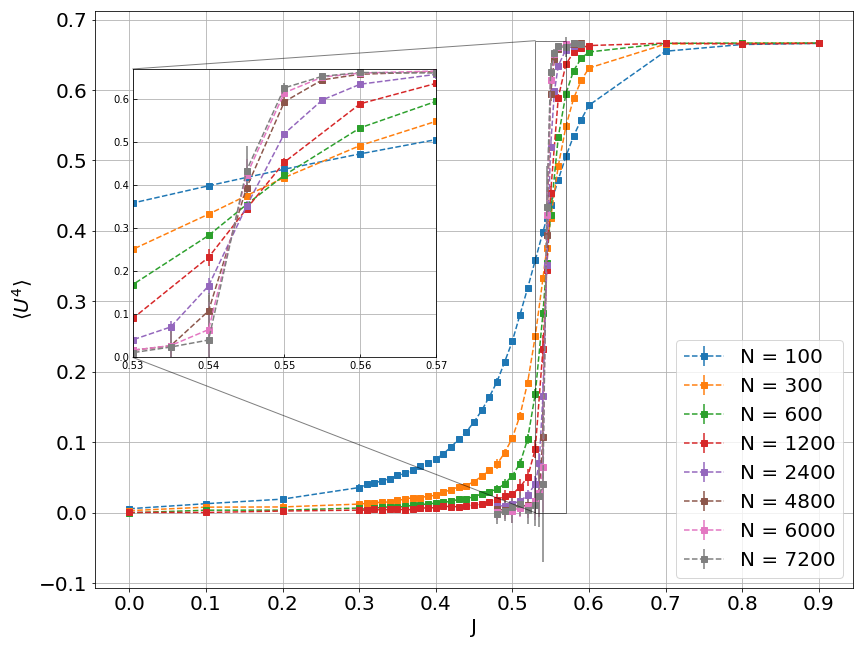
\includegraphics[width=\textwidth]{TrIsISAW_U4.png}
\caption{}
\label{fig:TrIsISAW_U4}
\end{subfigure}
\hfill
\begin{subfigure}{0.49\textwidth}
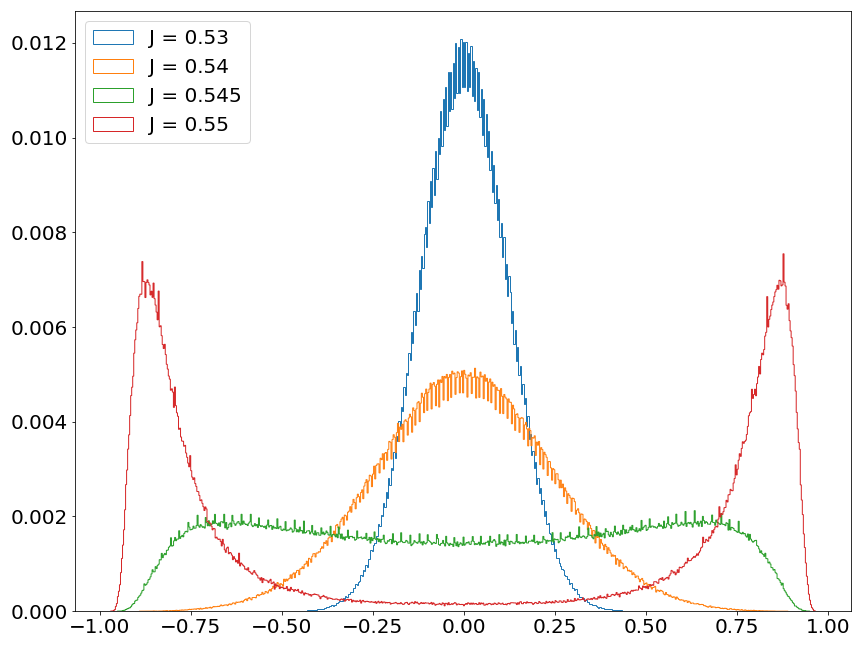
\includegraphics[width=\textwidth]{TrIsISAW_m2_distr.png}
\caption{}
\label{fig:TrIsISAW_m2_distr}
\end{subfigure}
\caption{Слева: кумулянт Биндера модели TrIsingISAW с длиной конформации от 100 до 7200 (длины отмечены разными цветами).
Справа: распределение удельной намагниченности модели TrIsingISAW на конформации длиной $N=7200$ при $J \in [0.53,0.55]$ (значения J отмечены разными цветами)}
\end{figure}


График \ref{fig:TrIsISAW_U4} показывает зависость кумулянта Биндера \eqref{eq:IsISAW_U4} от J. 
Пересечение графиков от конформаций разных длин, соответствующее переходу от парамагнетических к ферромагнетическим свойствам, снова наблюдается в $J \approx 0.545$.

Распределение значений удельной намагниченности для модели TrIsingISAW изображено на графике \ref{fig:TrIsISAW_m2_distr}.
График показывает, что распределение с преобладающими малыми по модулю значениями удельной намагниченности уступают 
распределениям с преобладающими крайними значениями намагниченности возле $J=0.545$, где распределение близко к почти равномерному.


\begin{figure}[h]
\begin{subfigure}{0.49\textwidth}
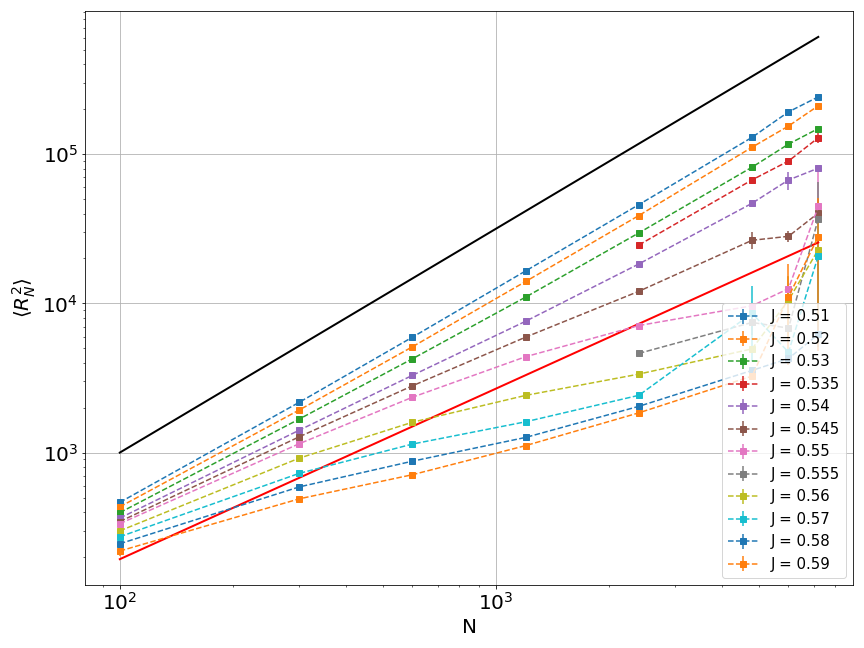
\includegraphics[width=\textwidth]{TrIsISAW_R2log.png}
\caption{}
\label{fig:TrIsISAW_R2log}
\end{subfigure}
\hfill
\begin{subfigure}{0.49\textwidth}
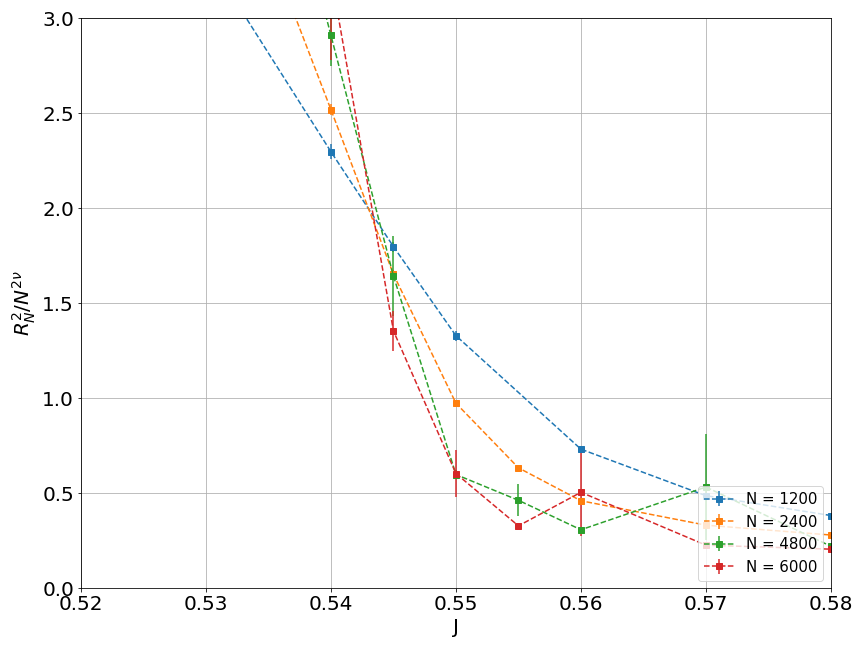
\includegraphics[width=\textwidth]{TrIsISAW_R2toN2v.png}
\caption{}
\label{fig:TrIsISAW_R2toN2v}
\end{subfigure}
\caption{Слева: Расстояние между концами блужданий длины $N$ при $J \in [0.51,0.59]$ в логарифмическом масштабе. 
Для наглядности добавлены линии $N^{2\nu}$, где $\nu = 4/7$ (красная линия) и $\nu=3/4$ (чёрная линия).
Справа: отношение расстояния между концами блуждания $R^2$ к $N^{2\nu}$, где $\nu=3/4$ при $J \in [0.52,0.58]$}
\end{figure}

Рассмотрим так же конформационный переход модели.
Рисунок \ref{fig:TrIsISAW_R2log} описывает расстояние между концами блужданий модели TrIsingISAW как функцию длины блуждания при фиксированном значении J.
Функции изображены в логарифмическом масштабе для наглядного наблюдения степенного шкалирования величины при $N \to \infty$.
Так же для сравнения были добавлены прямые $N^{2\nu}$, где $\nu = 4/7$ (красная линия) - константа поведения модели ISAW на квадратной решетке в точке критического перехода \cite{Duplantier1987},
и $\nu = 3/4$ (черная линия) - константа поведения невзаимодействующего блуждания без самопересечений \cite{Rensburg2015}.
На рисунке видно, что при $J \leq 0.53$ поведение графиков близко к чёрной линии, в то время как графики с $J = 0.54, 0.545$ в значительной степени схожи к красной линией.
У графиков с большим значением $J$, наблюдается сильное снижение наклона прямой, что говорит о более сжатом состоянии блужданий при $J \geq 0.55$.  

График \ref{fig:TrIsISAW_R2toN2v} описывает ту же величину, но перешкалированную относительно $N^{2\nu}$ в зависимости от $J$.
Результаты показывают, что вблизи точки $J = 0.543$ величина $R^2 / N^{2\nu}$ становится N-независимой. 

Таким образом, на основании пронаблюдаемых магнитного (рисунки \ref{fig:TrIsISAW_U4} и \ref{fig:TrIsISAW_m2_distr}) и конформационного (рисунок \ref{fig:TrIsISAW_R2log}) переходов,
точка фазового перехода модели предполагается возле точки $J=0.545$. Считая погрешностью оценки расстояние между измерениями, итоговая оценка точки фазового перехода:

\begin{equation}
\label{eq:TrIsISAW_Jc}
	J_c = 0.545(5)
\end{equation}

Для оценки критического кумулянта, ввиду слишком большой наблюдаемой погрешности, требуются более длительные симуляции длин $N > 5000$.


\newpage

\subsection{Критические экспоненты модели}

В данном подразделе критическое поведение модели TrIsingISAW будет исследовано в сравнении с оригинальной модификацией модели IsingISAW на квадратной решётке, рассмотренной ранее в статье \cite{faizullina2021critical}.
Прошкалируем наблюдаемые величины $\la R^2 \ra$ и $m^2$ относительно соотвествующих критических экспонент:
так, величины вблизи предполагаемой точки фазового перехода рассматриваются как функции:

\begin{equation}
\begin{array}{l}
\label{eq:TrIsISAW_datcoll}
\la R^2 \ra = N^{2\nu} f(x), \\
\la m^2 \ra = N^{-2\beta\phi} g(x), \\
x = (J-J_c) N^{\phi},
\end{array}
\end{equation}

где $\nu$, $\phi$, $\beta$  - пространственный, переходный, и порядковый показатели соответственно, в то время как $f(x)$ и $g(x)$ - безразменные шкалирующие функции безразмерной величины.
В рамках последующего анализа коллапса данных, подберём наилучшие критические показатели и точку фазового перехода, 
чтобы получить наиболее визуально гладкие функции $f(x)$ и $g(x)$ вблизи $x=0$.


\begin{figure}[h]
\begin{subfigure}{0.49\textwidth}
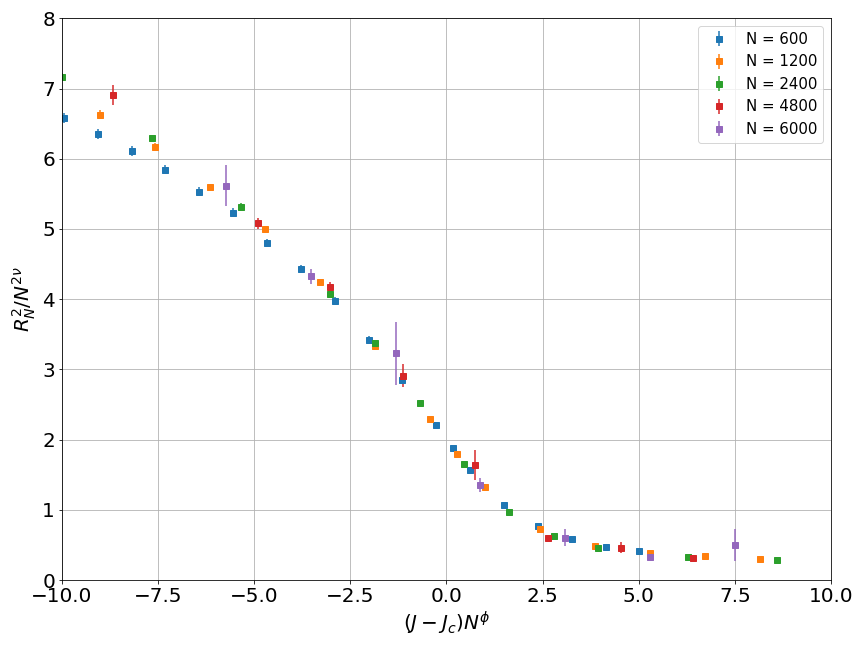
\includegraphics[width=\textwidth]{TrIsISAW_R2_datcoll.png}
\caption{}
\label{fig:TrIsISAW_R2_datcoll}
\end{subfigure}
\hfill
\begin{subfigure}{0.49\textwidth}
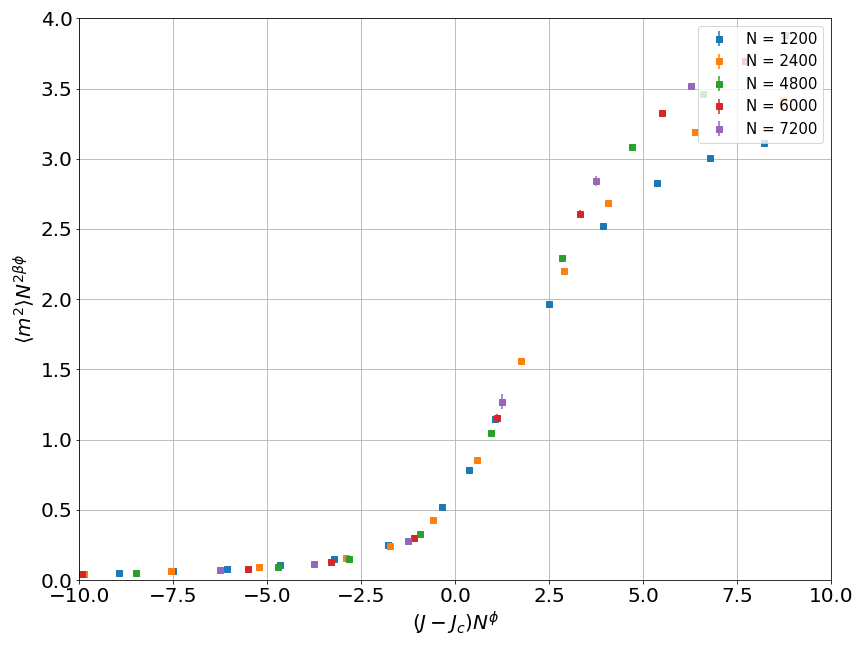
\includegraphics[width=\textwidth]{TrIsISAW_m2_datcoll.png}
\caption{}
\label{fig:TrIsISAW_m2_datcoll}
\end{subfigure}
\caption{Коллапс данных наблюдаемых величин модели TrIsingISAW.
Слева: Расстояние между концами блужданий $\la R^2_N \ra$, при $\nu = 4/7$, $\phi=0.7$, $J_c = 0.543$, N=[600, 6000].
Справа: Средняя вторая степень удельной магниченности $\la m^2 \ra$, при $\beta = 1/8$, $\phi=0.7$, $J_c = 0.5425$, N=[1200, 7200]}
\end{figure}

Графики \ref{fig:TrIsISAW_R2_datcoll} и \ref{fig:TrIsISAW_m2_datcoll} описывают наиболее гладко изображенные функции $f(x), g(x)$ \eqref{eq:TrIsISAW_datcoll}.
В качестве показателей были взяты результаты из работы \cite{faizullina2021critical}.
Результаты показывают, что использованные показатели при дополнительной коррекции точки фазового перехода $J_c$ дают достаточно чёткий коллапс данных.
Это подтвеждает универсальность критических экспонент родительских моделей Ising 2D (модель Изинга на двумерной решётке) 
и ISAW 2D (взаимодействующее бесспиновое случайное блуждание без самопересечений), из которых и были ранее взяты значения экспонент,
а также согласуется с оценкой критической точки выше \eqref{eq:TrIsISAW_Jc}.


\subsection{Вопросы}

\begin{itemize}
\item Статья 2021: что означает correction-to-scalling для графика $R^2 / N^{2\nu}$
\end{itemize}

